\begin{figure}[ht!]
\centering
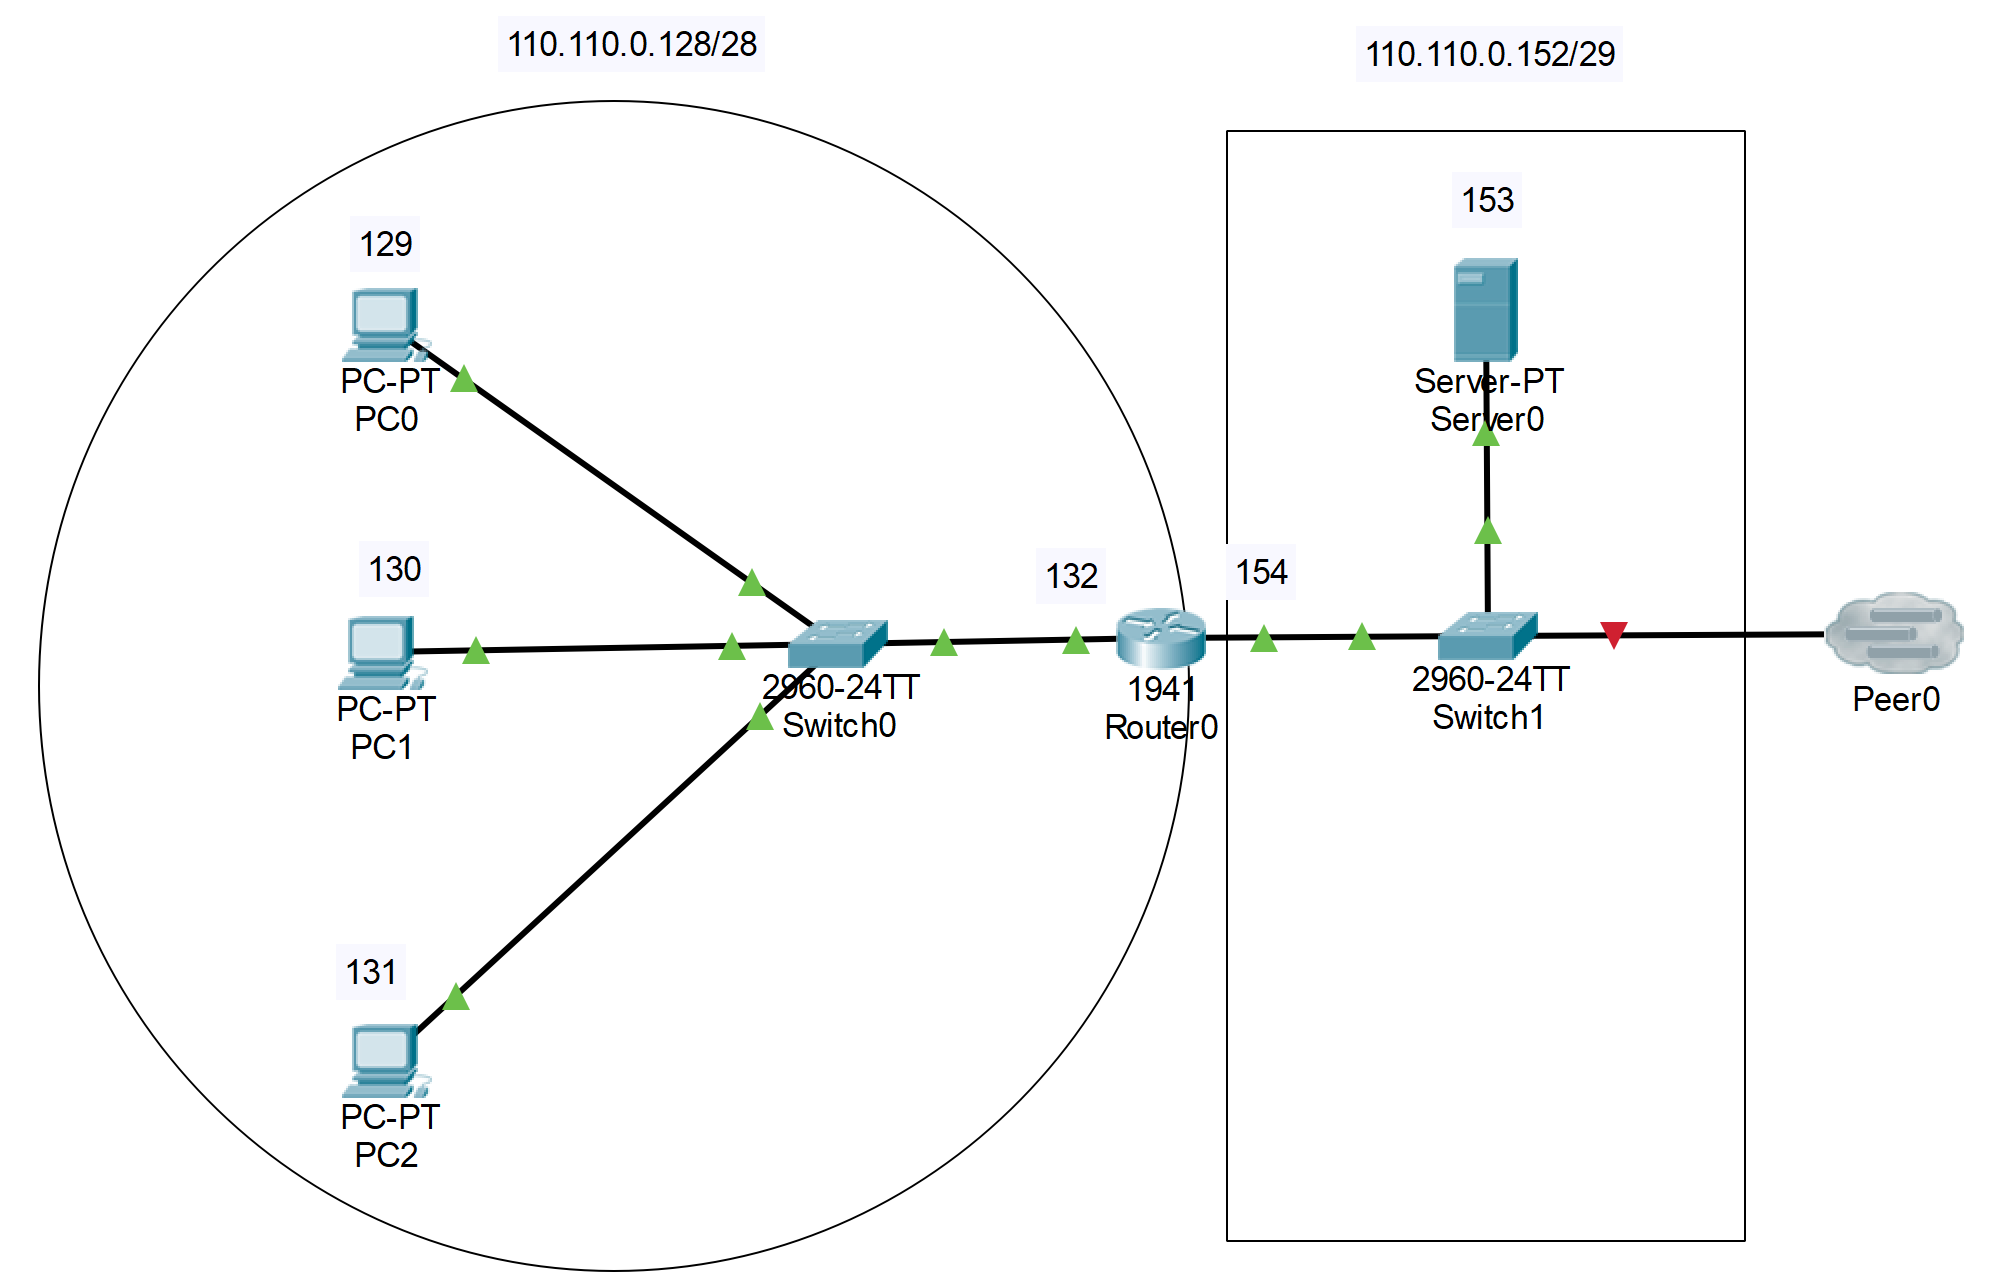
\includegraphics[scale=0.5]{Imagenes/net.png}
\end{figure}


\begin{enumerate}

\item {\color{red} La PC0 envía un paquete al servidor. ¿Como es el paquete que recibe el servidor? Dibujar a nivel ethernet.}

\begin{figure}[ht!]
\centering
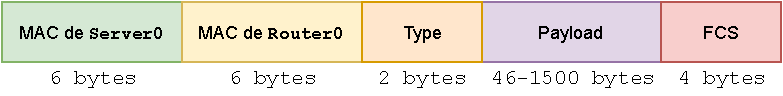
\includegraphics[scale=0.85]{Imagenes/ethernet.pdf}
\end{figure}

\item {\color{red} Explicar que es un Proxy ARP.}

Proxy ARP\cite{net} es una técnica mediante la cual un dispositivo proxy\footnote{Que actúa como puerta de enlace o intermediario entre cualquier dispositivo y el resto de Internet. Un proxy acepta y reenvía solicitudes de conexión, luego devuelve datos para esas solicitudes.} en una red determinada responde a las consultas ARP para una dirección IP que \textbf{no está en esa red}. El proxy es consciente de la ubicación del destino del tráfico y ofrece \textbf{su propia dirección MAC} como el destino (aparentemente final). El tráfico dirigido a la dirección del proxy normalmente es enrutado por el proxy al destino previsto a través de otra interfaz o mediante un túnel. \\

La principal ventaja de un ARP proxy es que puede usar un solo enrutador en una red para comunicarse con todas las máquinas de la red. la desventaja es que los hosts de la red piensan que todas las demás máquinas son accesibles mediante una solicitud ARP y luego aumentan la cantidad de información en sus tablas ARP.

\item {\color{red} ¿La PC0, puede conocer la dirección MAC del servidor a donde está el servicio requerido?}

A menos que el usuario de la \texttt{PC0} conozca la MAC del server y la haya colocado manualmente, \textbf{no}. Para eso se lleva a cabo el Address Resolution Protocol, así el remitente realiza una consulta ARP y esta le devuelve la dirección MAC del server o en otro caso la direccion MAC del router\cite{cisco}, en este caso el router se hace cargo del enrutamiento de los datos.

\end{enumerate}

\begin{thebibliography}{9}
\bibitem{cisco} 
Proxy ARP. Cisco \href{https://www.cisco.com/c/en/us/support/docs/ip/dynamic-address-allocation-resolution/13718-5.html}{https://www.cisco.com/c/en/us/support/docs/ip/dynamic-address-allocation-resolution/13718-5.html} January 28, 2008.

\bibitem{net} 
Proxy ARP,  Ed Harmoush \href{https://www.practicalnetworking.net/series/arp/proxy-arp/}{https://www.practicalnetworking.net/series/arp/proxy-arp/} January 16, 2017.

\bibitem{rfc}
Using ARP to Implement Transparent Subnet Gateways, RFC 1027
 \href{https://www.ietf.org/rfc/rfc1027.txt}{https://www.ietf.org/rfc/rfc1027.txt} 1987.

\bibitem{scientificsentence}
Address Resolution Protocol (ARP) \& Proxy ARP
 \href{https://scientificsentence.net/Networking/ARP.html\# :\~:text=Proxy\% 20ARP\% 20is\% 20the\% 20technique,from\% 20machines\% 20on\% 20a\% 20subnet}{https://scientificsentence.net/Networking/ARP.html\# :\~:text=Proxy\% 20ARP\% 20is\% 20the\% 20technique,from\% 20machines\% 20on\% 20a\% 20subnet}

\end{thebibliography}
